\documentclass[a4paper, 12pt]{article}
\usepackage{graphicx, xcolor, enumerate, geometry, times, CJK}

\title{SP HW10 report}
\author{Chih-Hsuan Yang(SCC)}

\begin{document}
\begin{CJK*}{UTF8}{bsmi}
  \maketitle
  \newpage

  \section{請畫出當資料數量固定為 1000,B=3,consumers 數量為 10、100、1000之折線圖。}
  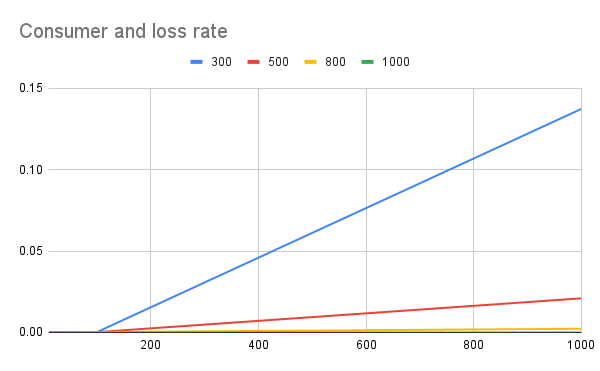
\includegraphics[width=\textwidth]{images/Consumer and loss rate.png}
  \label{fig1}

  \section{請畫出當資料數量固定為 1000,R=500,consumers 數量為 10、100、1000 之折線圖。}
  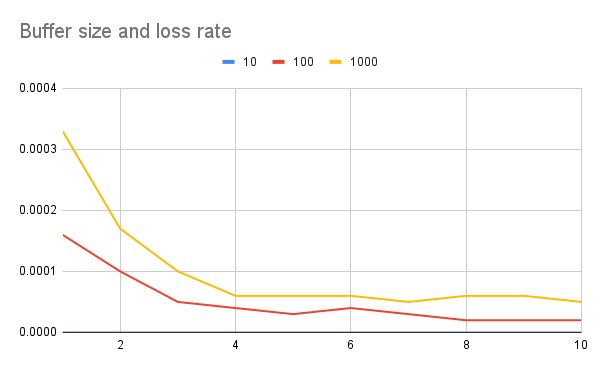
\includegraphics[width=\textwidth]{images/Buffer size and loss rate.png}

  \section{請描述您使用主機的作業系統、Memory、CPU。}
  \begin{enumerate}
    \item CPU: 11th Gen Intel i5-1135G7 (8) \@ 4.200GHz
    \item Memory: 39970MiB
    \item OS: Pop!\_OS 20.04 LTS x86\_64
    \item Host: Lemur Pro lemp10
    \item Kernel: 5.13.0-7620-generic
  \end{enumerate}

  \section{您覺得造成資料 loss 影響最大的因素為 Memory or CPU or buffer size?為什麼?}
  以上皆非,我們可以從上面兩張圖中看到,影響因素最大的是 context switch。
  瞥除 context switch 不談的話,是 memory 讀寫速度,因為我們可以從(圖 \ref{fig1}) 看出
  當 delay time (duration) 減少時,有些 process 可能會讀不到資料,造成 data loss。

  \section{另設計一個程式 (given fixed (M, B, R, N), 如:(1000, 3, 500, 150)),如何有
    效降低 Loss rate?}
  此版本採用 busy waiting 方式,各自即時 fetch data,已為最佳解。若要再漸低 lass rate 應從
  修改 kernel scheduler 著手,棌 polling 方式,並且設計較小 quantum time,再盡可能減少 context
  switch 上的成本。\\
  至於 PREEMPT\_RT 技術是否能夠應用於此場景,需要後續其他研究才能加以證明。

\end{CJK*}
\end{document}